% source-sha256: 66135b2d446ec88593e78b07e3f45c64e845bff835501e25b12cc5f48f23afd5
% Options for packages loaded elsewhere
\PassOptionsToPackage{unicode}{hyperref}
\PassOptionsToPackage{hyphens}{url}
\documentclass[
]{article}
\usepackage{xcolor}
\usepackage[letterpaper,margin=1in]{geometry}
\usepackage{amsmath,amssymb}
\setcounter{secnumdepth}{-\maxdimen} % remove section numbering
\usepackage{iftex}
\ifPDFTeX
  \usepackage[T1]{fontenc}
  \usepackage[utf8]{inputenc}
  \usepackage{textcomp} % provide euro and other symbols
\else % if luatex or xetex
  \usepackage{unicode-math} % this also loads fontspec
  \defaultfontfeatures{Scale=MatchLowercase}
  \defaultfontfeatures[\rmfamily]{Ligatures=TeX,Scale=1}
\fi
\usepackage{lmodern}
\ifPDFTeX\else
  % xetex/luatex font selection
\fi
% Use upquote if available, for straight quotes in verbatim environments
\IfFileExists{upquote.sty}{\usepackage{upquote}}{}
\IfFileExists{microtype.sty}{% use microtype if available
  \usepackage[]{microtype}
  \UseMicrotypeSet[protrusion]{basicmath} % disable protrusion for tt fonts
}{}
\makeatletter
\@ifundefined{KOMAClassName}{% if non-KOMA class
  \IfFileExists{parskip.sty}{%
    \usepackage{parskip}
  }{% else
    \setlength{\parindent}{0pt}
    \setlength{\parskip}{6pt plus 2pt minus 1pt}}
}{% if KOMA class
  \KOMAoptions{parskip=half}}
\makeatother
\usepackage{color}
\usepackage{fancyvrb}
\newcommand{\VerbBar}{|}
\newcommand{\VERB}{\Verb[commandchars=\\\{\}]}
\DefineVerbatimEnvironment{Highlighting}{Verbatim}{commandchars=\\\{\}}
% Add ',fontsize=\small' for more characters per line
\newenvironment{Shaded}{}{}
\newcommand{\AlertTok}[1]{\textcolor[rgb]{1.00,0.00,0.00}{\textbf{#1}}}
\newcommand{\AnnotationTok}[1]{\textcolor[rgb]{0.38,0.63,0.69}{\textbf{\textit{#1}}}}
\newcommand{\AttributeTok}[1]{\textcolor[rgb]{0.49,0.56,0.16}{#1}}
\newcommand{\BaseNTok}[1]{\textcolor[rgb]{0.25,0.63,0.44}{#1}}
\newcommand{\BuiltInTok}[1]{\textcolor[rgb]{0.00,0.50,0.00}{#1}}
\newcommand{\CharTok}[1]{\textcolor[rgb]{0.25,0.44,0.63}{#1}}
\newcommand{\CommentTok}[1]{\textcolor[rgb]{0.38,0.63,0.69}{\textit{#1}}}
\newcommand{\CommentVarTok}[1]{\textcolor[rgb]{0.38,0.63,0.69}{\textbf{\textit{#1}}}}
\newcommand{\ConstantTok}[1]{\textcolor[rgb]{0.53,0.00,0.00}{#1}}
\newcommand{\ControlFlowTok}[1]{\textcolor[rgb]{0.00,0.44,0.13}{\textbf{#1}}}
\newcommand{\DataTypeTok}[1]{\textcolor[rgb]{0.56,0.13,0.00}{#1}}
\newcommand{\DecValTok}[1]{\textcolor[rgb]{0.25,0.63,0.44}{#1}}
\newcommand{\DocumentationTok}[1]{\textcolor[rgb]{0.73,0.13,0.13}{\textit{#1}}}
\newcommand{\ErrorTok}[1]{\textcolor[rgb]{1.00,0.00,0.00}{\textbf{#1}}}
\newcommand{\ExtensionTok}[1]{#1}
\newcommand{\FloatTok}[1]{\textcolor[rgb]{0.25,0.63,0.44}{#1}}
\newcommand{\FunctionTok}[1]{\textcolor[rgb]{0.02,0.16,0.49}{#1}}
\newcommand{\ImportTok}[1]{\textcolor[rgb]{0.00,0.50,0.00}{\textbf{#1}}}
\newcommand{\InformationTok}[1]{\textcolor[rgb]{0.38,0.63,0.69}{\textbf{\textit{#1}}}}
\newcommand{\KeywordTok}[1]{\textcolor[rgb]{0.00,0.44,0.13}{\textbf{#1}}}
\newcommand{\NormalTok}[1]{#1}
\newcommand{\OperatorTok}[1]{\textcolor[rgb]{0.40,0.40,0.40}{#1}}
\newcommand{\OtherTok}[1]{\textcolor[rgb]{0.00,0.44,0.13}{#1}}
\newcommand{\PreprocessorTok}[1]{\textcolor[rgb]{0.74,0.48,0.00}{#1}}
\newcommand{\RegionMarkerTok}[1]{#1}
\newcommand{\SpecialCharTok}[1]{\textcolor[rgb]{0.25,0.44,0.63}{#1}}
\newcommand{\SpecialStringTok}[1]{\textcolor[rgb]{0.73,0.40,0.53}{#1}}
\newcommand{\StringTok}[1]{\textcolor[rgb]{0.25,0.44,0.63}{#1}}
\newcommand{\VariableTok}[1]{\textcolor[rgb]{0.10,0.09,0.49}{#1}}
\newcommand{\VerbatimStringTok}[1]{\textcolor[rgb]{0.25,0.44,0.63}{#1}}
\newcommand{\WarningTok}[1]{\textcolor[rgb]{0.38,0.63,0.69}{\textbf{\textit{#1}}}}
\setlength{\emergencystretch}{3em} % prevent overfull lines
\providecommand{\tightlist}{%
  \setlength{\itemsep}{0pt}\setlength{\parskip}{0pt}}
% Release-document layout safeguards injected by scripts/generate_docs.sh.
\usepackage{fvextra}
\fvset{breaklines=true,breakanywhere=true,fontsize=\small}
\RecustomVerbatimEnvironment{verbatim}{Verbatim}{breaklines=true,breakanywhere=true,fontsize=\small}
\setlength{\emergencystretch}{3em}
\AtBeginDocument{\sloppy}
% Workflow-figure support: mermaid blocks in the canonical Markdown are mapped
% to hand-authored TikZ figures by scripts/pandoc_bounded_tables.lua.
\usepackage{tikz}
\usetikzlibrary{shapes.geometric,arrows.meta,positioning,fit,backgrounds,calc}
\definecolor{bdiStep}{HTML}{EAF2FB}
\definecolor{bdiEdge}{HTML}{365F91}
\definecolor{bdiText}{HTML}{17253A}
\definecolor{bdiGate}{HTML}{FFF5D6}
\definecolor{bdiGateEdge}{HTML}{9B6B00}
\definecolor{bdiOpt}{HTML}{F0EAF7}
\definecolor{bdiOptEdge}{HTML}{5B3E86}
\definecolor{bdiOut}{HTML}{E6F4EA}
\definecolor{bdiOutEdge}{HTML}{1E6B3A}
\tikzset{
  bdi/.style={draw=bdiEdge,line width=1pt,fill=bdiStep,text=bdiText,rounded corners=3pt,
              align=center,inner sep=4pt,font=\scriptsize\sffamily},
  bdigate/.style={bdi,draw=bdiGateEdge,fill=bdiGate},
  bdiopt/.style={bdi,draw=bdiOptEdge,fill=bdiOpt,dashed},
  bdiout/.style={bdi,draw=bdiOutEdge,fill=bdiOut},
  bdiflow/.style={-{Stealth[length=2mm]},draw=bdiEdge,line width=0.9pt},
  bdiback/.style={bdiflow,dashed},
  bdilbl/.style={font=\tiny\sffamily,text=bdiText,inner sep=1.5pt,fill=white},
}
\usepackage{bookmark}
\IfFileExists{xurl.sty}{\usepackage{xurl}}{} % add URL line breaks if available
\urlstyle{same}
% fallback for those not using the hyperref driver hyperxmp:
\makeatletter
\@ifundefined{xmpquote}{\newcommand{\xmpquote}[1]{#1}}{}
\makeatother
\hypersetup{
  pdftitle={Business Document Ingestion},
  pdfauthor={Christopher Melhauser and theonlymuffinbot},
  hidelinks,
  pdfcreator={LaTeX via pandoc}}

\title{Business Document Ingestion}
\usepackage{etoolbox}
\makeatletter
\providecommand{\subtitle}[1]{% add subtitle to \maketitle
  \apptocmd{\@title}{\par {\large #1 \par}}{}{}
}
\makeatother
\subtitle{Client User Guide}
\author{Christopher Melhauser and theonlymuffinbot}
\date{September 3, 2026}

\begin{document}
\maketitle

\section{Before you send documents}\label{before-you-send-documents}

\subsection{Authorship and AI collaboration
context}\label{authorship-and-ai-collaboration-context}

Courtesy credit is given to Christopher Melhauser and
\texttt{theonlymuffinbot}. Here, \texttt{theonlymuffinbot} describes
collaborative AI tooling. This identifies the tooling context and does
not assign legal authorship or ownership to an AI system.

\subsection{Operator readiness}\label{operator-readiness}

\subsubsection{Optional image-submission
workflow}\label{optional-image-submission-workflow}

If your engagement enables the visual-intake pilot, you can submit
original PNG or JPEG page images through a compatible application for
the connected vision-capable assistant to read. This is separate from
the ordinary PDF delivery below and from the approved reporting
database. Agree the source set, provider data flow, ownership and
retention location first. The operator must also satisfy the existing
MCP deployment gate; intake is not enabled by default.

Keep originals unchanged. The current limit is 1 to 20 declared pages
per session, 10,000,000 original bytes and 25,000,000 pixels per image.
Direct PDF, HEIC, WebP, animation and URL uploads are not supported. The
application must transfer real bytes; do not assume a photograph
attached to chat has reached the service. Smaller deployment request
limits may apply. No capture app or attachment relay is supplied by this
repository.

Retain the session ID and every upload/proposal receipt outside the
chat. Ask the assistant to discover the schema, read all retained pages,
cite their locations, preserve unfamiliar labels and identify uncertain
values. Even a valid result is \textbf{pending review, not published}.
An unreadable or rejected page stays visible. Corrections create another
proposal, not an edit to an approved account/contact/invoice. Retry an
uncertain request with exactly the same key and content; changed content
needs a new key. Replacing an already retained source page requires a
new session, preserving the old one.

For processing, an authorized local operator exports the session to a
new private source archive, verifies it against the separately retained
receipt, and inspects the complete derived image PDF before normal
profiling/intake. The archive retains every original attempt, proposal
version and rejection, with a page map and review exceptions. A blocked
archive or partial PDF must not advance. Normal independent extraction,
business controls, authorization and final review remain required before
any new approved snapshot or CRM file.

See \href{../references/visual-ingestion.md}{Visual Intake} for exact
tools, flags, permissions and recovery, and
\href{CLIENT_OUTPUT_OVERVIEW.md}{Client Output Overview} for everyday
queries, reports and the distinction between source and CRM exports.

\subsubsection{Standard pipeline provider
preparation}\label{standard-pipeline-provider-preparation}

For a Google-backed run, the operator should refresh credentials
immediately before a live run:

\begin{Shaded}
\begin{Highlighting}[]
\ExtensionTok{python}\NormalTok{ scripts/reauthorize\_google.py}
\end{Highlighting}
\end{Shaded}

The helper asks for the GCP project, refreshes both gcloud login and
Vertex AI Application Default Credentials, verifies that tokens can be
issued, and can prepare a temporary Document AI token file. Credentials
and tokens stay outside the repository and must never be included with
client documents or run output. If
\texttt{GOOGLE\_\allowbreak{}APPLICATION\_\allowbreak{}CREDENTIALS} is
set, confirm that its external file is current; otherwise Vertex AI uses
the refreshed local ADC.

\begin{enumerate}
\def\labelenumi{\arabic{enumi}.}
\tightlist
\item
  Keep the original files unchanged. Do not rename, split, rotate, or
  combine pages after delivery unless you also retain the original copy.
\item
  Send PDFs in the order you received them. A single PDF with many pages
  is acceptable; the process creates one output file per source page.
\item
  Include your reference exports when available: purchase orders, jobs,
  projects, account codes, general ledger, payments, and remittance
  records.
\item
  Tell us the date range, document types you expect, currency or
  currencies, and the business questions you want answered.
\item
  Flag any material privacy, retention, residency, or access
  restrictions.
\end{enumerate}

\subsection{Recommended delivery
structure}\label{recommended-delivery-structure}

Place the delivery materials in four clearly labelled folders or files:

\begin{itemize}
\tightlist
\item
  \texttt{source\_\allowbreak{}pdfs/\allowbreak{}} --- original PDFs; no
  edited replacements;
\item
  \texttt{reference\_\allowbreak{}exports/\allowbreak{}} --- purchase
  order, job, project, or other approved business references;
\item
  \texttt{accounting\_\allowbreak{}exports/\allowbreak{}} ---
  general-ledger, payment, and remittance data when available; and
\item
  \texttt{delivery\_\allowbreak{}notes.txt} --- date range, known
  issues, and requested outcomes.
\end{itemize}

If a source PDF has multiple pages, do not split it yourself. The
process keeps the delivered PDF as a byte-identical, SHA-256-verified
source copy and creates an ordered, one-page output for each page.

\section{What happens after delivery}\label{what-happens-after-delivery}

\begin{enumerate}
\def\labelenumi{\arabic{enumi}.}
\tightlist
\item
  Every page is profiled and retained.
\item
  Pages are placed in sorted, one-page output files.
\item
  The process proposes multi-page groups only when page markers,
  document type, and business identifiers agree. It can also surface an
  unordered same-type / unique-ID candidate, clearly marked for
  page-order review rather than assembled automatically.
\item
  Extracted values are checked for agreement, mathematical consistency,
  and business-format rules.
\item
  Uncertain, handwritten, duplicate, missing, or conflicting evidence is
  collected for review.
\end{enumerate}

\subsection{Process flow and the optional AI
layer}\label{process-flow-and-the-optional-ai-layer}

\textbf{Original PDFs and references} → \textbf{immutable intake} →
\textbf{independent proposals} → \textbf{consensus, proof, and
validation} → \textbf{final client-review gate} → \textbf{reporting or
agreed load handoff}.

When the gate is open, the client supplies a confirmation, correction,
or cited evidence. The operator records an amendment or decision and
regenerates the gate. Optional AI output always enters this same path;
it never closes the gate.

\begin{figure}[htbp]
\centering
\resizebox{\ifdim\width>\textwidth\textwidth\else\width\fi}{!}{%
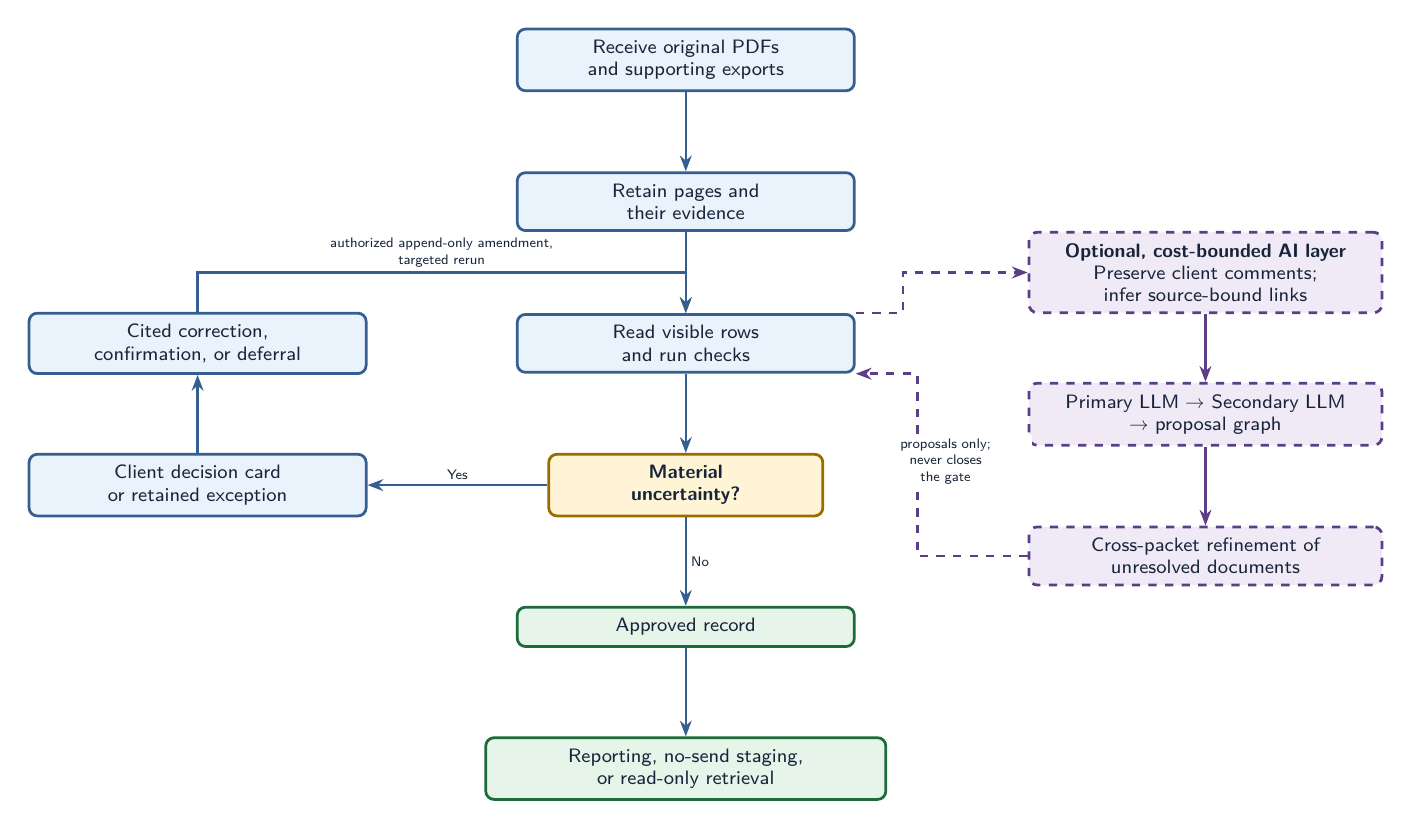
\begin{tikzpicture}[x=1mm,y=1mm]
  % Deterministic spine.
  \node[bdi,text width=40mm] (A) at (0,0)    {Receive original PDFs\\and supporting exports};
  \node[bdi,text width=40mm] (B) at (0,-18)  {Retain pages and\\their evidence};
  \node[bdi,text width=40mm] (C) at (0,-36)  {Read visible rows\\and run checks};
  \node[bdigate,text width=32mm] (D) at (0,-54) {\textbf{Material\\uncertainty?}};
  \node[bdiout,text width=40mm] (G) at (0,-72) {Approved record};
  \node[bdiout,text width=48mm] (H) at (0,-90) {Reporting, no-send staging,\\or read-only retrieval};

  % Client decision path, to the left.
  \node[bdi,text width=40mm] (F) at (-62,-36) {Cited correction,\\confirmation, or deferral};
  \node[bdi,text width=40mm] (E) at (-62,-54) {Client decision card\\or retained exception};

  \draw[bdiflow] (A)--(B);
  \draw[bdiflow] (B)--(C);
  \draw[bdiflow] (C)--(D);
  \draw[bdiflow] (D)--node[bdilbl,right]{No}(G);
  \draw[bdiflow] (G)--(H);
  \draw[bdiflow] (D)--node[bdilbl,above]{Yes}(E);
  \draw[bdiflow] (E)--(F);
  % The amendment return path is routed above the row so its label sits clear of
  % both the decision box it leaves and the extraction box it re-enters.
  \draw[bdiflow] (F.north) -- ++(0,5) coordinate (m)
        -- node[bdilbl,above,align=center,text width=50mm]
           {authorized append-only amendment,\\targeted rerun}
           (m -| C.north) -- (C.north);

  % Optional AI layer, to the right.
  \node[bdiopt,text width=42mm] (I) at (66,-27) {\textbf{Optional, cost-bounded AI layer}\\Preserve client comments;\\infer source-bound links};
  \node[bdiopt,text width=42mm] (J) at (66,-45) {Primary LLM $\rightarrow$ Secondary LLM\\$\rightarrow$ proposal graph};
  \node[bdiopt,text width=42mm] (K) at (66,-63) {Cross-packet refinement of\\unresolved documents};

  \draw[bdiflow,draw=bdiOptEdge] (I)--(J);
  \draw[bdiflow,draw=bdiOptEdge] (J)--(K);
  \draw[bdiback,draw=bdiOptEdge] (C.north east) -- ++(6,0) |- (I.west);
  \draw[bdiback,draw=bdiOptEdge] (K.west) -- ++(-14,0) |- (C.south east);
  \node[bdilbl,align=center,text width=21mm] at (33,-51)
        {proposals only;\\never closes\\the gate};
\end{tikzpicture}
}
\caption{The client decision and amendment lifecycle. Optional AI output re-enters the same review path as everything else and can never close the gate.}
\end{figure}

The AI step is optional and cost-bounded. Address parsing is local by
default. If an approved run enables external address validation, each
unique address may be sent within a stated cap of no more than 5,000
calls per run; the result is a deliverability and geographic proposal,
never a replacement for the original. The configured LLM preserves a raw
response and page hash, returns document-type and likely
handwriting-region proposals and review flags, and is never the only
reader or final decision-maker. The image-preparation stage keeps
grayscale, contrast-enhanced, and complementary black-and-white copies
for comparison; none replaces the original page. A separately enabled
LLM adjudication lane may assess only explicit, printed, nonfinancial
candidates after deterministic validation and independent agreement. Its
confidence floor defaults to \texttt{0.99} and may be adjusted from
\texttt{0.99} to \texttt{1.0}; it still creates a clearly audit-marked
amendment proposal for client review, never a client-approved record.

An optional card-level client-review assistant can summarize all
supplied extractor, schema, arithmetic, validation, entity, and
handwriting evidence. It may identify low-risk review items that depend
on another item, but it never approves facts or deletes findings. The
retained output contains every original item; only a clearly labelled
client-facing view may collapse an explicitly covered dependency.
Protected financial, handwriting, arithmetic, provider, identity, and
reassembly findings remain visible.

Each item may also include an evidence-backed
\texttt{llm\_\allowbreak{}proposed\_\allowbreak{}update} with the
original value, proposed value, field, evidence, and rationale. A
separate cross-record phase may find supporting evidence elsewhere in
the supplied run. Both are proposals only. A thresholded carry-forward
is disabled by default, and
\texttt{scripts/\allowbreak{}simulate\_\allowbreak{}client\_\allowbreak{}approval.py}
is reserved for simulation-only stress tests; it cannot approve
production facts or populate retrieval.

The final review stage can use a separately configured LLM. All other
client-review controls are inherited from the current run, and the
selected provider and model are retained in the internal audit metadata.

\subsubsection{AI-assisted draft comments are not client
decisions}\label{ai-assisted-draft-comments-are-not-client-decisions}

An operator may generate an optional companion review workbook using an
AI simulated-client reviewer. Every comment is visibly labelled
\textbf{``AI client reviewed (simulated; not client authorization)''}
and includes its model, source-visible evidence quote, and raw-response
audit reference. It is a way to prepare a reasoned draft and to identify
the items that deserve your attention; it does not speak for you, change
your workbook, approve a record, or close a review item. Financial,
identity, arithmetic, provider, reassembly, and other protected findings
always remain human review work.

The reviewer keeps item-specific source citations, an interruption-safe
checkpoint, and explicit exceptions. An interrupted run may resume only
when its queue, evidence, and configuration hashes still match. Any
later retry is a separate retained overlay; prior comments and failures
are never overwritten.

If you wish to use the draft, compare each proposed recommendation with
the original source and make your actual decision in the returned review
workbook. We preserve both the issued and returned workbooks, retain the
AI companion package separately, compile your decisions, apply only
separately authorized append-only changes, and rerun the affected
controls. Missing ledger or payment evidence is not cured by an AI
draft.

For a multi-year statement corpus, the optional table-comprehension lane
retains one evidence-linked source-row proposal per page. Later pages
may provide layout context--headers, sections, totals, and template
fingerprints only--for bounded rereads of uncertain earlier pages. Any
changed reading becomes a linked amendment proposal. When an initial
audit identifies a concern, Google Document AI may provide a
page-matched buddy check; financial, identity, handwriting, mapping, and
reassembly issues still remain in the final review package.

\subsection{Mapping names and
locations}\label{mapping-names-and-locations}

If a source uses an unfamiliar label, the system proposes a standard
business meaning and places it in the review package. It does not
silently add a new field or reuse that proposal for another layout. Once
you approve a mapping, it is versioned for that exact layout; a later
header, dealer name, brand name, relationship, or city change is
reviewed again. Names and relationships are kept with their effective
history.

An address printed on a page can be validated separately. If the
document only gives a dealer or brand name, the optional Google Places
check can provide possible locations. It is a short candidate list for
your review, not an automatic match or replacement address. Approved,
provenance-linked records can then be delivered as a vendor-neutral CRM
staging package with no-send CSV/API instructions and a citation-backed
retrieval database. An optional verified no-send package also reshapes
approved facts into common account, contact, address, product,
transaction, shipment, and payment CSVs, with a target-mapping worksheet
and write/reconciliation plan. Those files do not authorize an upload:
the client CRM team must validate the actual tenant fields and keys,
approve the mapping, prove idempotency and rollback in a sandbox, and
separately authorize the exact production package. The database can be
queried through local read-only MCP, an explicitly enabled TLS-only
bearer REST API, or the separately deployed OAuth-protected remote MCP
for approved Claude or ChatGPT mobile/web/desktop access. The remote MCP
can create bounded, expiring, checksummed CSV/XLSX downloads from
approved tables or standard reports. Selecting a target CRM and
accepting public hosting, identity-provider, workspace, privacy,
retention, and user-access controls remain separate client decisions;
none of these read-only interfaces writes to a CRM.

\subsection{Commission and sales-credit
review}\label{commission-and-sales-credit-review}

Some commission reports include multiple allocations for one order. The
process preserves each allocation separately, calculates its effective
commission rate from the reported commission and commissionable amount,
and retains any printed rate or allocation share as evidence. An
explicitly approved policy can classify a low-rate/ship-to allocation as
administrative and exclude it from sales credit, while treating a
qualifying sales allocation separately.

If the rate or rule differs by brand, dealer, product, client, location,
or date, the client receives one short decision card per report policy.
The client only edits the decision return file---not the report, the
source evidence, or the historical registry---and can specify the scope
and dates. A new rule creates a later version; earlier results remain
traceable. Unfamiliar layers or unclear formulas remain in the normal
final-review package.

\section{Privacy and delivery
controls}\label{privacy-and-delivery-controls}

The process can produce a privacy inventory of obvious sensitive
patterns in retained text without changing your originals. Tell us your
access, residency, retention, and redaction requirements before
delivery. Do not send passwords, API keys, or credentials in document
packages.

\subsection{The smaller client review
package}\label{the-smaller-client-review-package}

For a grouped review, the client package is limited to three files:
\texttt{client\_\allowbreak{}review\_\allowbreak{}package.xlsx},
\texttt{client\_\allowbreak{}review\_\allowbreak{}guide.docx}, and
\texttt{decision\_\allowbreak{}pages.docx}. The workbook has an
Executive Summary, a Decisions Needed sheet with one drop-down choice
for each client decision, and Representative Cards. The guide explains
the review in everyday language. The decision pages show one
representative source-page reference for each choice.

The package does not include the internal appendix, drill-down, raw
provider evidence, or exhaustive item list. Those records remain
retained internally. Complete \texttt{Your\ choice} and
\texttt{Your\ note} only, leave
\texttt{Internal\ only\ —\ no\ client\ choice} rows unchanged, and
return a separate copy of the workbook. The operator preserves the
issued workbook unchanged and imports the returned copy with
\texttt{scripts/\allowbreak{}client\_\allowbreak{}review\_\allowbreak{}package.py import-\allowbreak{}decisions}
and the exact issued workbook path. The importer verifies every group
and fixed cell against that issued copy and records both workbook
hashes. The result is a proposal and still goes through the normal
final-review controls; it never applies a production fact directly.
Before repairing or reissuing a legacy package, preserve the returned
choices and notes with
\texttt{scripts/\allowbreak{}client\_\allowbreak{}review\_\allowbreak{}package.py preserve-\allowbreak{}responses}.
This creates a separate proposal-only JSON snapshot without changing
either workbook, so no client response is lost while lineage or contract
issues are resolved.

\section{Reviewing the final package}\label{reviewing-the-final-package}

The v1.0 delivery keeps each run in a new output location so an earlier
manifest, provider handoff, privacy inventory, or review package is not
silently replaced. You will receive the canonical
\texttt{final\_\allowbreak{}client\_\allowbreak{}review.json} package.
It is accompanied by these reviewer views:

\begin{itemize}
\tightlist
\item
  \texttt{final\_\allowbreak{}client\_\allowbreak{}review.csv} --- a
  spreadsheet-friendly list.
\item
  \texttt{final\_\allowbreak{}client\_\allowbreak{}review.xlsx} --- a
  formatted, filterable Excel workbook.
\item
  \texttt{final\_\allowbreak{}client\_\allowbreak{}review.html} --- a
  browser-friendly review view.
\end{itemize}

The JSON package is the canonical record; the reviewer views are
convenience copies. Each item identifies the document, page, field or
handwriting region, reason, and priority. The Excel workbook includes
\texttt{Client\ Review} for filtering, plus
\texttt{Header\ Definitions}, \texttt{Schema\ Definitions}, and
\texttt{Runbook} so it can be understood without another file. The
separate \texttt{examples/\allowbreak{}} folder contains only artefacts
marked \textbf{SAMPLE - FICTIONAL - NOT CLIENT DATA}; they illustrate
field shapes and are not review decisions or client data.

For each item, choose one of these outcomes:

\begin{itemize}
\tightlist
\item
  Confirm the displayed value or grouping.
\item
  Provide the corrected value, with the supporting page or system
  reference.
\item
  Mark the item as not applicable, with a reason.
\item
  Provide a missing reference, payment, or ledger record.
\end{itemize}

Corrections are recorded as amendments. The original page and original
reading remain available for audit.

\subsection{How to return a decision}\label{how-to-return-a-decision}

Use the JSON \texttt{document\_\allowbreak{}id},
\texttt{page\_\allowbreak{}id}, \texttt{region\_\allowbreak{}id} (if
shown), \texttt{field}, and \texttt{reason} to identify the item. Return
the outcome with a citation to the source page or business system. Do
not edit the JSON, CSV, or workbook as if that changed the original
record: the operator creates a new amendment and regenerates the final
package.

\subsection{Step-by-step client return and rerun
checklist}\label{step-by-step-client-return-and-rerun-checklist}

This checklist explains what to do with the three operator artifacts
supplied after a workbook return. A returned choice is evidence for a
proposal; it is not an automatic production change.

\begin{figure}[htbp]
\centering
\resizebox{\ifdim\width>\textwidth\textwidth\else\width\fi}{!}{%
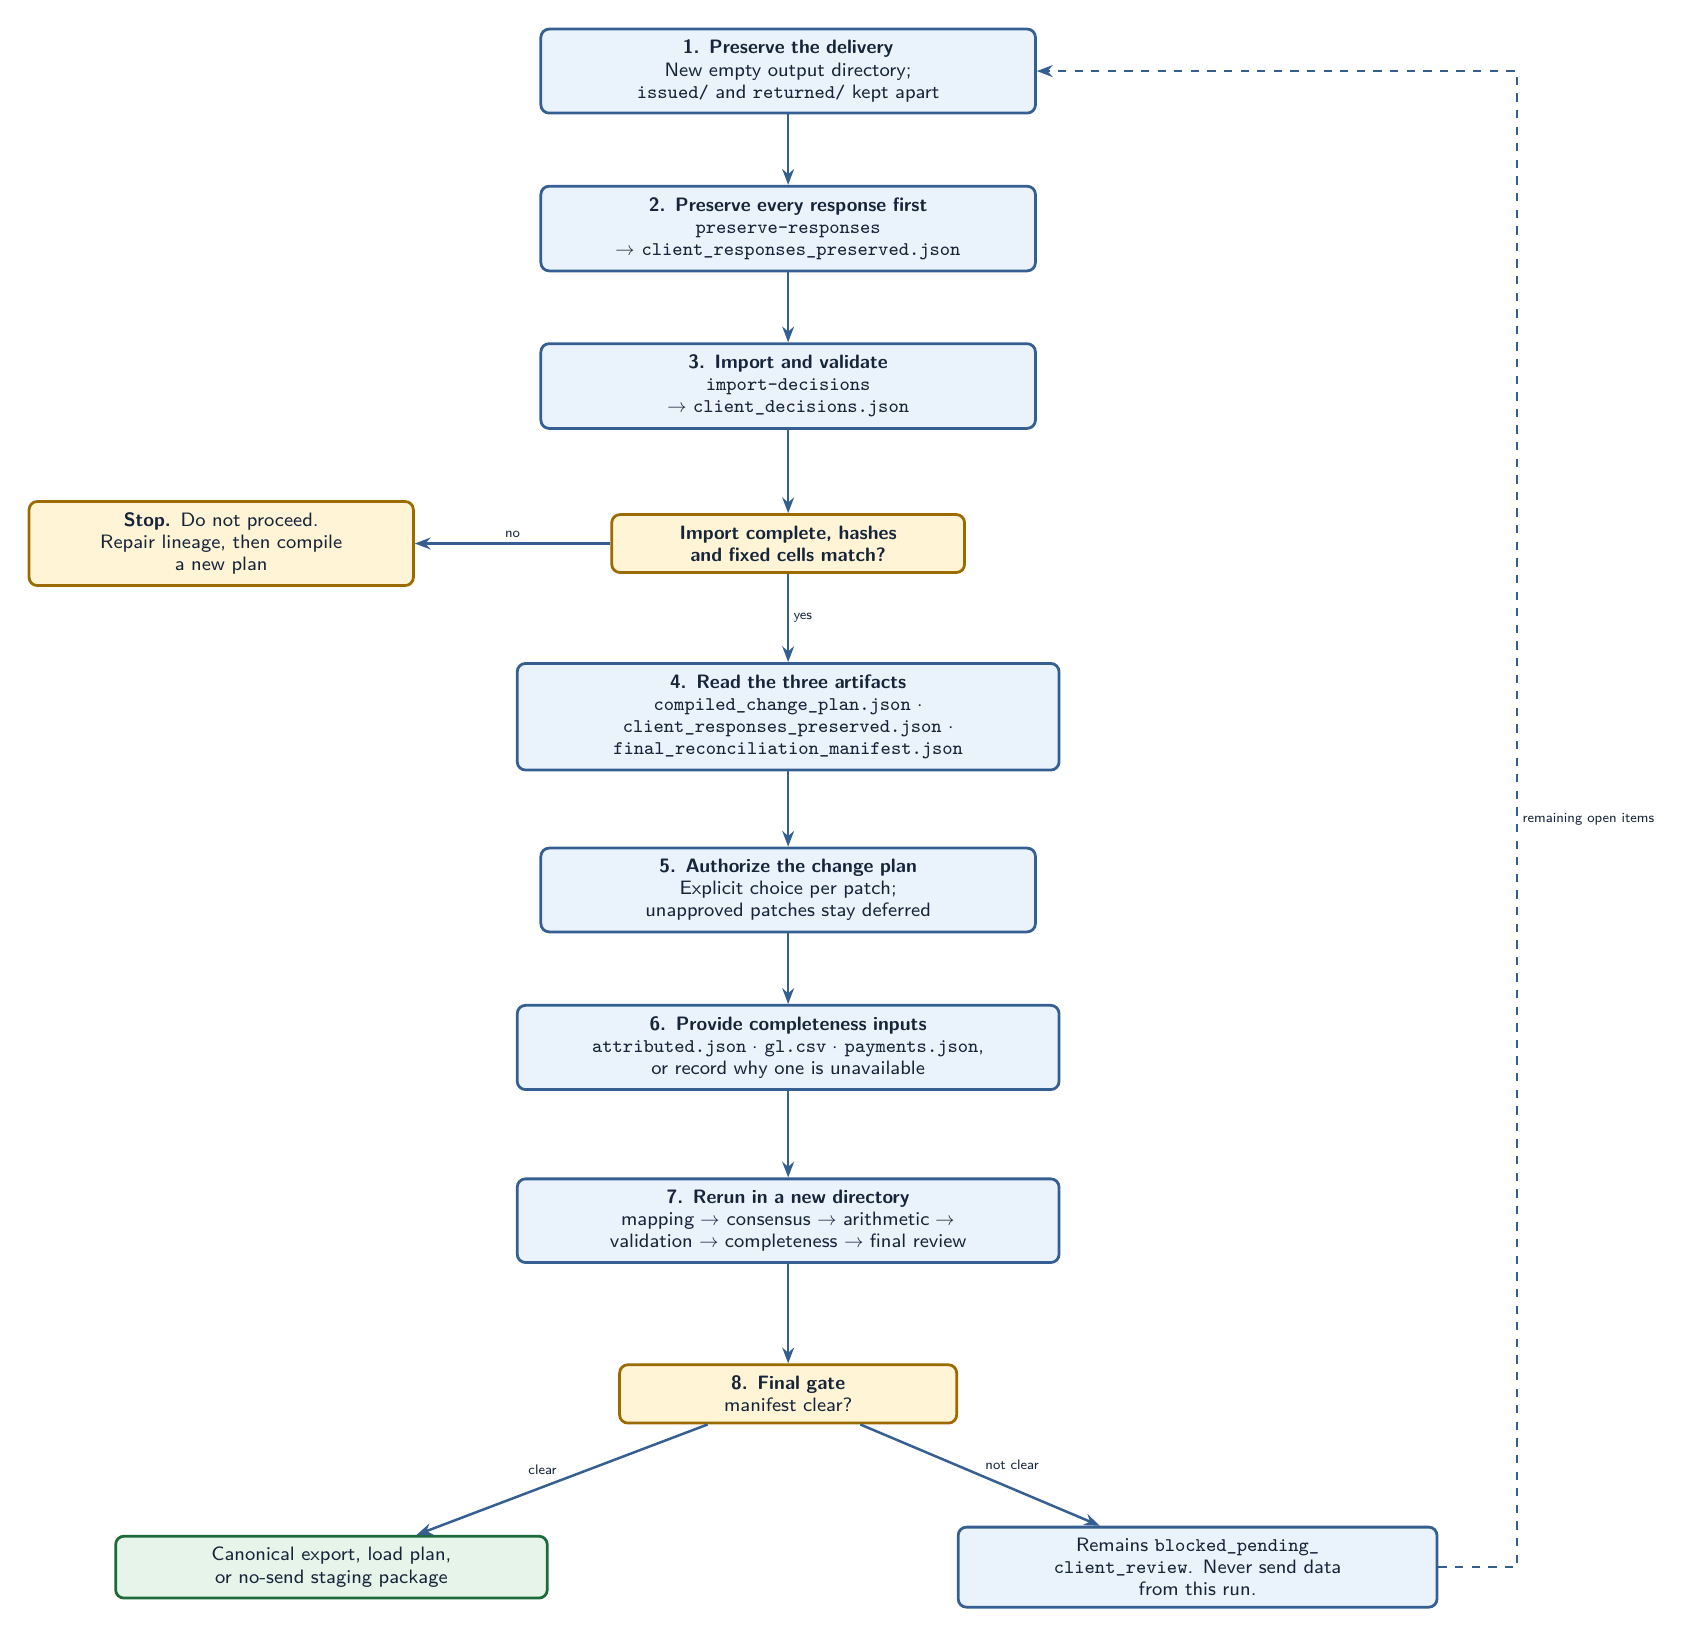
\begin{tikzpicture}[x=1mm,y=1mm]
  \node[bdi,text width=60mm] (S1) at (0,0)    {\textbf{1. Preserve the delivery}\\New empty output directory;\\\texttt{issued/} and \texttt{returned/} kept apart};
  \node[bdi,text width=60mm] (S2) at (0,-20)  {\textbf{2. Preserve every response first}\\\texttt{preserve-responses}\\$\rightarrow$ \texttt{client\_responses\_preserved.json}};
  \node[bdi,text width=60mm] (S3) at (0,-40)  {\textbf{3. Import and validate}\\\texttt{import-decisions}\\$\rightarrow$ \texttt{client\_decisions.json}};
  \node[bdigate,text width=42mm] (V) at (0,-60) {\textbf{Import complete, hashes\\and fixed cells match?}};
  \node[bdigate,text width=46mm] (STOP) at (-72,-60) {\textbf{Stop.} Do not proceed.\\Repair lineage, then compile\\a new plan};
  \node[bdi,text width=66mm] (S4) at (0,-82)  {\textbf{4. Read the three artifacts}\\\texttt{compiled\_change\_plan.json} $\cdot$\\\texttt{client\_responses\_preserved.json} $\cdot$\\\texttt{final\_reconciliation\_manifest.json}};
  \node[bdi,text width=60mm] (S5) at (0,-104) {\textbf{5. Authorize the change plan}\\Explicit choice per patch;\\unapproved patches stay deferred};
  \node[bdi,text width=66mm] (S6) at (0,-124) {\textbf{6. Provide completeness inputs}\\\texttt{attributed.json} $\cdot$ \texttt{gl.csv} $\cdot$ \texttt{payments.json},\\or record why one is unavailable};
  \node[bdi,text width=66mm] (S7) at (0,-146) {\textbf{7. Rerun in a new directory}\\mapping $\rightarrow$ consensus $\rightarrow$ arithmetic $\rightarrow$\\validation $\rightarrow$ completeness $\rightarrow$ final review};
  \node[bdigate,text width=40mm] (S8) at (0,-168) {\textbf{8. Final gate}\\manifest clear?};
  \node[bdiout,text width=52mm] (OK) at (-58,-190) {Canonical export, load plan,\\or no-send staging package};
  \node[bdi,text width=58mm] (NO) at (52,-190) {Remains \texttt{blocked\_pending\_}\\\texttt{client\_review}. Never send data\\from this run.};

  \foreach \a/\b in {S1/S2,S2/S3,S3/V,S4/S5,S5/S6,S6/S7,S7/S8}{\draw[bdiflow] (\a)--(\b);}
  \draw[bdiflow] (V)--node[bdilbl,above]{no}(STOP);
  \draw[bdiflow] (V)--node[bdilbl,right]{yes}(S4);
  \draw[bdiflow] (S8)--node[bdilbl,above left]{clear}(OK);
  \draw[bdiflow] (S8)--node[bdilbl,above right]{not clear}(NO);
  \draw[bdiback] (NO.east) -- ++(10,0)
        |- node[bdilbl,pos=0.25,right]{remaining open items} (S1.east);
\end{tikzpicture}
}
\caption{The eight-step client return and rerun sequence. Each step is a separate gate: preservation precedes import, compilation precedes authorization, and authorization precedes any production change.}
\end{figure}

\subsubsection{1. Preserve the delivery}\label{preserve-the-delivery}

Create a new, empty output directory for this return. Copy the issued
workbook and returned workbook into separate
\texttt{issued/\allowbreak{}} and \texttt{returned/\allowbreak{}}
folders. Keep both copies unchanged and never overwrite an earlier run.

\subsubsection{2. Preserve every response
first}\label{preserve-every-response-first}

Run this before importing or repairing the workbook:

\begin{Shaded}
\begin{Highlighting}[]
\ExtensionTok{python}\NormalTok{ scripts/client\_review\_package.py preserve{-}responses }\DataTypeTok{\textbackslash{}}
\NormalTok{  returned/client\_review\_revised.xlsx }\DataTypeTok{\textbackslash{}}
  \AttributeTok{{-}{-}issued{-}workbook}\NormalTok{ issued/client\_review\_package.xlsx }\DataTypeTok{\textbackslash{}}
  \AttributeTok{{-}{-}out}\NormalTok{ client\_responses\_preserved.json}
\end{Highlighting}
\end{Shaded}

Treat
\texttt{client\_\allowbreak{}responses\_\allowbreak{}preserved.json} as
an audit snapshot. Check its \texttt{response\_\allowbreak{}count},
decision-group IDs, and mismatch status. Do not edit it.

\subsubsection{3. Import and validate the returned
workbook}\label{import-and-validate-the-returned-workbook}

\begin{Shaded}
\begin{Highlighting}[]
\ExtensionTok{python}\NormalTok{ scripts/client\_review\_package.py import{-}decisions }\DataTypeTok{\textbackslash{}}
\NormalTok{  returned/client\_review\_revised.xlsx }\DataTypeTok{\textbackslash{}}
  \AttributeTok{{-}{-}issued{-}workbook}\NormalTok{ issued/client\_review\_package.xlsx }\DataTypeTok{\textbackslash{}}
  \AttributeTok{{-}{-}out}\NormalTok{ client\_decisions.json}
\end{Highlighting}
\end{Shaded}

Stop if the import is incomplete, any decision is invalid, groups are
missing or reordered, fixed cells changed, or workbook hashes do not
match. Confirm that the response set in
\texttt{client\_\allowbreak{}decisions.json} matches the preserved
snapshot. Neither file changes source evidence or approves a canonical
fact.

\subsubsection{4. Use the three artifacts for their separate
purposes}\label{use-the-three-artifacts-for-their-separate-purposes}

\begin{itemize}
\tightlist
\item
  \texttt{compiled\_\allowbreak{}change\_\allowbreak{}plan.json}: review
  the proposed patches, deferred decisions, affected fields/documents,
  and rerun lanes. This is the artifact to use when deciding what may be
  authorized.
\item
  \texttt{client\_\allowbreak{}responses\_\allowbreak{}preserved.json}:
  prove that every client choice and note was retained unchanged. It is
  an audit record, not an editing surface.
\item
  \texttt{final\_\allowbreak{}reconciliation\_\allowbreak{}manifest.json}:
  check the current gate, completeness blockers, arithmetic status,
  retained evidence, and required next stages. It determines whether the
  run may advance.
\end{itemize}

\subsubsection{5. Authorize the change
plan}\label{authorize-the-change-plan}

Review each proposed patch in the compiled plan. Complete the separate
operator-authorization template with the operator identity, timestamp,
and an explicit choice for every patch; leave unapproved patches
deferred. A lineage or contract exception may permit proposal
compilation, but never authorizes production application. Bind the
completed authorization to the unchanged plan:

\begin{Shaded}
\begin{Highlighting}[]
\ExtensionTok{python}\NormalTok{ scripts/client\_decision\_compile.py authorize }\DataTypeTok{\textbackslash{}}
\NormalTok{  compiled\_change\_plan.json operator\_authorization\_completed.json }\DataTypeTok{\textbackslash{}}
  \AttributeTok{{-}{-}out}\NormalTok{ authorized\_change\_plan.json}
\end{Highlighting}
\end{Shaded}

If any plan, workbook-lineage, or catalog hash changes, stop and compile
a new plan rather than editing the existing one.

\subsubsection{6. Provide the completeness
inputs}\label{provide-the-completeness-inputs}

Provide the applicable \texttt{attributed.json}, \texttt{gl.csv}, and
\texttt{payments.json}, or record explicitly why one is unavailable.
These are required for attribution, GL variance, payment/aging closure,
and completeness. Missing evidence keeps the gate blocked; it must not
be inferred from an LLM proposal.

These files have distinct roles:

\begin{itemize}
\tightlist
\item
  \texttt{attributed.json} is the pipeline's derived attribution result.
  It links each in-scope monetary record to an ACK, job, project, or
  other approved business reference, with the evidence chain; unresolved
  amounts remain in its unattributable register. The operator generates
  it from the validated/proofed records and the client's reference
  export; the client should not hand-edit it.
\item
  \texttt{gl.csv} is the client's authoritative general-ledger export.
  It is used to compare document totals by accounting period and report
  variances. The completeness command also accepts an equivalent JSON GL
  export when that is the client's native format.
\item
  \texttt{payments.json} is the client's authoritative payment or
  remittance export. CSV is accepted too, so send whatever the finance
  system exports rather than converting it by hand. It supports
  invoice/payment matching, partial-payment handling, and aging closure.
  Any row that cannot be matched to an invoice number is reported back
  to you rather than skipped. Preserve the original export and its
  source-system/date metadata.
\end{itemize}

Send these exports with the column headings your system already prints.
A heading such as \texttt{Job\ \#}, \texttt{ACK\ No.}, or
\texttt{Invoice\ Number} is matched as written; you do not need to
rename columns, and renaming them edits the evidence before we read it.
Any row we cannot use is returned to you with its original heading and
content rather than being dropped.

These are reference/control artifacts, not replacement copies of the
source PDFs and not client-review answers. If \texttt{attributed.json}
has not yet been generated, supply the ACK/job/project reference export
and the operator will run the attribution stage before completeness.

If the client has no GL or payment export, the operator may create
clearly labelled \textbf{inferred proposal} artifacts from retained
document evidence. Those artifacts must record their inference method,
source documents, missing fields, and confidence/exception counts. They
can prioritize review, but they are not accounting or payment-system
evidence and cannot change the completeness gate to \texttt{clear}. The
final manifest must retain the missing authoritative control as an
explicit exception unless the client later supplies or approves an
authoritative substitute.

For a repeatable proposal run, use the retained consensus/proofed
artifact and a new output directory:

\begin{Shaded}
\begin{Highlighting}[]
\ExtensionTok{python}\NormalTok{ scripts/inferred\_controls.py consensus.json }\DataTypeTok{\textbackslash{}}
  \AttributeTok{{-}{-}out{-}dir}\NormalTok{ inferred\_controls\_proposal\_YYYYMMDDTHHMMSSZ}
\end{Highlighting}
\end{Shaded}

This produces \texttt{attributed.json}, \texttt{gl.csv},
\texttt{payments.json}, \texttt{exceptions.json}, and a hash-bound
\texttt{manifest.json}. The manifest records
\texttt{blocked\_\allowbreak{}inferred\_\allowbreak{}controls\_\allowbreak{}not\_\allowbreak{}authoritative};
do not rename or remove that status.

When authoritative reference, ledger, or payment exports are
unavailable, a second, optional lane can use the preserved client review
only as bounded reasoning context. First create a hash-bound context
bundle from the preserved responses and a deterministic pilot of
retained records:

\begin{Shaded}
\begin{Highlighting}[]
\ExtensionTok{python}\NormalTok{ scripts/client\_review\_context.py client\_responses\_preserved.json }\DataTypeTok{\textbackslash{}}
  \AttributeTok{{-}{-}records}\NormalTok{ consensus\_superseding.json }\AttributeTok{{-}{-}max{-}documents}\NormalTok{ 75 }\DataTypeTok{\textbackslash{}}
  \AttributeTok{{-}{-}out}\NormalTok{ client\_review\_context.json}
\end{Highlighting}
\end{Shaded}

If you provided comments in a separate JSON, CSV, TSV, TXT, Markdown, or
PDF file, give the unchanged original to the operator. The operator
preserves and hashes it with:

\begin{Shaded}
\begin{Highlighting}[]
\ExtensionTok{python}\NormalTok{ scripts/client\_input\_comments.py client\_notes.json client\_followup.csv }\DataTypeTok{\textbackslash{}}
  \AttributeTok{{-}{-}records}\NormalTok{ consensus\_superseding.json }\DataTypeTok{\textbackslash{}}
  \AttributeTok{{-}{-}out}\NormalTok{ client\_input\_comments\_context.json}
\end{Highlighting}
\end{Shaded}

For CSV or TSV you do not have to format anything: a spreadsheet of
notes is read as it is, with each non-empty row taken as one comment and
nothing treated as a heading to be thrown away. If you would rather
label the columns, name the note column
\texttt{client\_\allowbreak{}comment}, \texttt{comment},
\texttt{comments}, \texttt{note}, \texttt{notes}, or \texttt{text}, and
optional document/page/field columns then help the LLM find the relevant
source. For JSON, use a list of comment strings/objects or an object
containing \texttt{comments{[}{]}}. TXT and Markdown treat each
non-empty line as a comment. The system preserves the original wording
and source-file hash. These comments help the LLM understand
terminology, priorities, and questions, but they do not become source
evidence, authorization, or approval.

Then run the disabled-by-default reference-discovery pilot with the
configured Primary LLM:

\begin{Shaded}
\begin{Highlighting}[]
\ExtensionTok{python}\NormalTok{ scripts/client\_review\_inference.py client\_review\_context.json }\DataTypeTok{\textbackslash{}}
  \AttributeTok{{-}{-}enable} \DataTypeTok{\textbackslash{}}
  \AttributeTok{{-}{-}out}\NormalTok{ reference\_discovery.json }\DataTypeTok{\textbackslash{}}
  \AttributeTok{{-}{-}exceptions}\NormalTok{ reference\_discovery\_exceptions.json }\DataTypeTok{\textbackslash{}}
  \AttributeTok{{-}{-}raw{-}dir}\NormalTok{ reference\_discovery\_raw}
\end{Highlighting}
\end{Shaded}

The context bundle preserves every client response and marks comments as
untrusted, reasoning-only context. The LLM may propose only
source-visible ACK/job/project/PO/invoice/order/payment/check/remittance
references or links; every proposal must cite a document and evidence
quote. Raw requests and responses, model metadata, retries, and schema
failures are retained. This lane cannot create GL or payment
transactions, approve attribution, clear completeness/aging, enter
independent consensus, or replace client evidence. When enabled, each
batch receives one bounded same-provider self-check by default. This
catches unsupported document IDs and evidence quotes, but it is not
independent consensus and cannot establish accounting evidence. Review
and authorize each surviving proposal through the normal append-only
workflow, then rerun the affected controls. Set the
\texttt{CLIENT\_\allowbreak{}REVIEW\_\allowbreak{}CONTEXT\_\allowbreak{}LLM\_\allowbreak{}*}
flags in \texttt{.env} for a repeatable bounded pilot;
\texttt{.env.example} documents every flag.

For the repeatable iterative lane, the Primary LLM proposes
source-backed relationships and the independently configured Secondary
LLM checks them. Run it in a fresh directory:

\begin{Shaded}
\begin{Highlighting}[]
\ExtensionTok{python}\NormalTok{ scripts/client\_review\_iterative.py client\_review\_context.json }\DataTypeTok{\textbackslash{}}
  \AttributeTok{{-}{-}primary{-}out}\NormalTok{ iterative\_primary.json }\DataTypeTok{\textbackslash{}}
  \AttributeTok{{-}{-}buddy{-}out}\NormalTok{ iterative\_buddy.json }\DataTypeTok{\textbackslash{}}
  \AttributeTok{{-}{-}exceptions}\NormalTok{ iterative\_exceptions.json }\AttributeTok{{-}{-}raw{-}dir}\NormalTok{ iterative\_raw }\DataTypeTok{\textbackslash{}}
  \AttributeTok{{-}{-}records}\NormalTok{ consensus\_superseding.json }\AttributeTok{{-}{-}iterations}\NormalTok{ 3 }\DataTypeTok{\textbackslash{}}
  \AttributeTok{{-}{-}convergence{-}min{-}new{-}candidates}\NormalTok{ 1}
\end{Highlighting}
\end{Shaded}

The lane adapts batch boundaries to the serialized packet size and
records a batch-scoped exception with the exact
\texttt{source\_\allowbreak{}document\_\allowbreak{}ids} for any source
item that still cannot fit or whose provider retries are exhausted; it
never silently drops that item. Retries are deliberately bounded. After
the run, use those IDs to create a fresh, no-clobber recovery run; an
item that remains unresolved is an explicit review exception, not a
successful inference.

The Secondary LLM labels proposals \texttt{confirmed},
\texttt{close\_\allowbreak{}needs\_\allowbreak{}review},
\texttt{conflict}, or \texttt{unsupported}. \texttt{confirmed} and
\texttt{close\_\allowbreak{}needs\_\allowbreak{}review} are final-guess
proposals only; neither status is authorization. Increase
\texttt{-\/-iterations} only when a prior round leaves useful
source-bound hypotheses to test; the implementation hard cap is five and
the configured default is three. A later pass stops automatically when
it adds no new source-backed, buddy-confirmed relationship (or fewer
than the configured convergence minimum). Every request and raw response
is retained, and each round is provenance-bound to the context hash.

After the in-packet passes, use the graph-guided cross-packet lane for
two separate safeguards. It discovers links for documents without an
in-packet buddy candidate, and independently verifies already-resolved
proposals against other retained documents that share a printed business
identifier, such as an ACK, invoice, PO, job, project, payment,
remittance, payee, or party reference. It never uses client comments as
proof. A cross-packet verification can flag an existing proposal as
close, conflicting, or unsupported; it never deletes or silently changes
the original proposal. Documents with no usable cross-packet evidence
and cap-deferred verification items are explicit exceptions:

The default neighborhood contains up to 6 documents and 80,000
serialized bytes. This is a moderate throughput setting; reduce it for
tighter quotas or increase it only after confirming provider context and
rate limits.

\begin{Shaded}
\begin{Highlighting}[]
\ExtensionTok{python}\NormalTok{ scripts/client\_review\_cross\_packet.py client\_review\_context.json }\DataTypeTok{\textbackslash{}}
  \AttributeTok{{-}{-}records}\NormalTok{ consensus\_superseding.json }\DataTypeTok{\textbackslash{}}
  \AttributeTok{{-}{-}primary}\NormalTok{ iterative\_primary.json }\AttributeTok{{-}{-}buddy}\NormalTok{ iterative\_buddy.json }\DataTypeTok{\textbackslash{}}
  \AttributeTok{{-}{-}graph}\NormalTok{ evidence\_graph.json }\DataTypeTok{\textbackslash{}}
  \AttributeTok{{-}{-}max{-}verification{-}neighborhoods}\NormalTok{ 100 }\DataTypeTok{\textbackslash{}}
  \AttributeTok{{-}{-}max{-}iterations}\NormalTok{ 2 }\AttributeTok{{-}{-}convergence{-}min{-}new{-}candidates}\NormalTok{ 1 }\DataTypeTok{\textbackslash{}}
  \AttributeTok{{-}{-}out}\NormalTok{ cross\_packet\_proposals.json }\DataTypeTok{\textbackslash{}}
  \AttributeTok{{-}{-}exceptions}\NormalTok{ cross\_packet\_exceptions.json }\AttributeTok{{-}{-}raw{-}dir}\NormalTok{ cross\_packet\_raw}
\end{Highlighting}
\end{Shaded}

The default cross-packet run permits two passes. Its follow-up pass
includes only newly exposed unresolved neighborhoods from material
relationships in the previous pass, and stops when it no longer finds a
material new relationship. The output is a separate proposal overlay
with both new candidates and verification records. Rebuild the evidence
graph with the new artifact before any further bounded refinement; do
not overwrite the prior graph or treat a cross-packet match or
verification as authorization.

Before the cross-packet package is finalized, the operator freezes the
completed pass and runs a separate retry pass for every
provider-retryable exception. The retry output is reconciled with the
original output and all remaining data or coverage exceptions stay
visible. This retry step is append-only and does not replace the
original responses.

The deterministic JSON evidence graph can then be built and queried with
\texttt{evidence\_\allowbreak{}graph.py build}, \texttt{query},
\texttt{path}, \texttt{candidates}, and \texttt{contradictions}. When a
run has retained non-consensus field readings, the operator can also use
\texttt{schema-surface\ -\/-consensus} to list those candidates---such
as source-visible addresses or labeled contact/representative
details---beside their source pointers. This is a completeness aid for
review: it does not accept the reading, assign a person a role, or
change a graph edge. Graph edges and LLM proposals remain protected
until an authorized append-only change is applied.

If the inventory identifies a small, relevant subset, the operator can
create a separate recovery scope for addresses or label-bound
contact/representative evidence. That scope lists exact source pages for
a fresh, independently checked overlay; it does not rerun the corpus,
change the original result, or treat an inferred role as approved.

\subsubsection{7. Rerun in a new
directory}\label{rerun-in-a-new-directory}

After authorization, apply only the authorized append-only changes and
rerun the affected lanes, followed by downstream controls in this order:
(1) classification and mapping, (2) independent primary and secondary
consensus, (3) arithmetic, (4) deterministic validation, (5)
entity/attribution/payment/ completeness checks, and (6) exhaustive
final review and package generation. Retain every original value, raw
response, exception, source index, and evidence link. Batch decisions
cannot clear protected arithmetic, provider, reassembly, handwriting,
identity, missing-field, or unresolved-evidence findings.

\subsubsection{8. Confirm the final gate}\label{confirm-the-final-gate}

Advance only when the final manifest is \texttt{clear}, applicable
completeness and arithmetic gates pass, protected findings are resolved
or explicitly retained as exceptions, and the regenerated package still
contains all client responses. Only then create a canonical export, load
plan, no-send CRM/API staging package, or common CRM import package.
Never send data from a proposal-only or
\texttt{blocked\_\allowbreak{}pending\_\allowbreak{}client\_\allowbreak{}review}
run.

\section{Handwritten notes and
signatures}\label{handwritten-notes-and-signatures}

Handwritten numbers are treated more carefully than printed text. A
financial handwritten change always needs your review, even when
independent systems agree. Signatures are retained as evidence and are
not converted into a person name.

\section{When the review gate is
clear}\label{when-the-review-gate-is-clear}

When the final review package is clear and reconciliation requirements
have been met, the approved records can move to reporting or to the
agreed business-system load process. A clear review package does not
replace your approval of the business outcome; it confirms that the
supplied control artifacts contain no unresolved issue. It is exhaustive
only for the source artifacts listed inside that package. The delivery
should also include the applicable run manifest, completeness report,
unattributable register, sampling decision, and client decision records.

For a plain-language walkthrough of the delivered files, record lookup,
reporting, MCP/API connection choices, controlled CSV/XLSX downloads,
and CRM-ready input packages, read
\href{CLIENT_OUTPUT_OVERVIEW.md}{\texttt{CLIENT\_\allowbreak{}OUTPUT\_\allowbreak{}OVERVIEW.md}}.

\section{Need help?}\label{need-help}

If an item is unclear, respond with the document/page identifier in the
review package and the source evidence that supports your decision. Do
not edit the source PDF in place; send an additional note or revised
evidence instead.

For a suspected credential, privacy, or evidence-integrity incident,
stop the affected optional provider step and use the private reporting
path in the delivered \texttt{SECURITY.md}. Do not place client data or
credentials in a public issue.

\subsection{Image quality, handwriting, and unordered
pages}\label{image-quality-handwriting-and-unordered-pages}

The process may prepare several comparison copies of a difficult page
and use an optional vision proposal to point out a likely handwritten
area. When the Google handwriting OCR lane is approved, it reads every
retained page and binds its proposed text only to those separately
identified regions. Google is one reader, not its own validator. Each
region and reading shares a stable page region ID so text cannot be
attached by list order or a nearby label; numeric handwriting still
requires unanimous agreement from three independent provider groups, and
financial handwriting still comes back for review. The process may also
identify a possible unordered page match. None of these actions changes
your source document or makes an approval; unclear cases are included in
the final review package.

\end{document}
